The equation of line joining A and B is given by 
\begin{align}
    \vec{r} &= \vec{A}+\lambda(\vec{B}-\vec{A})   
\end{align}
General equation of plane is given by
\begin{align}
    \vec{n}^T\vec{r} = c
\end{align}
where $\vec{n}$ is normal vector to the plane 
\begin{align}
    \vec{n} = \myvec{n_1\\n_2\\n_3}
\end{align}
\begin{lemma}
    The point of intersection of line
    \begin{align}
        \vec{r} &= \vec{A}+\lambda(\vec{B}-\vec{A})
    \end{align}
    and plane
    \begin{align}
        \vec{n}^T\vec{r} = c  
    \end{align}
    is given by
    \begin{align}
        \vec{r_0} = \vec{A}+\brak{\frac{c-\vec{n}^T\vec{A}}{\vec{n}^T(\vec{B}-\vec{A})}}(\vec{B}-\vec{A})
    \end{align}
\end{lemma}
\begin{proof}
Let $r_0$ be the point of intersection of the line and the plane then the point lies on both line and plane so,
\begin{align}
    \vec{r_0} &= \vec{A}+\lambda(\vec{B}-\vec{A})  
\end{align}
As $r_0$ also lies on plane
\begin{align}
    &\vec{n}^T\vec{r_0} = c\\
    \implies &\vec{n}^T(\vec{A}+\lambda(\vec{B}-\vec{A})) = c\\
    \implies &\lambda\vec{n}^T(\vec{B}-\vec{A}) = c-\vec{n}^T\vec{A}\\
    \implies &\lambda = \brak{\frac{c-\vec{n}^T\vec{A}}{\vec{n}^T(\vec{B}-\vec{A})}}
\end{align}
Therefore,
\begin{align}
    \vec{r_0} = \vec{A}+\brak{\frac{c-\vec{n}^T\vec{A}}{\vec{n}^T(\vec{B}-\vec{A})}}(\vec{B}-\vec{A})
\end{align}
\end{proof}
Given,
\begin{align}
    \vec{A} = \myvec{5\\1\\6}\\
    \vec{B} = \myvec{3\\4\\1}
\end{align}
Equation of line joining A and B is given by 
\begin{align}
    \vec{r} &= \vec{A}+\lambda(\vec{B}-\vec{A})\\
\end{align}
Equation of ZX-plane is given by
\begin{align}
    &y=0\\
    \implies &\vec{n}=\myvec{0\\1\\0}, c=0
\end{align}
Therefore coordinates of the intersection point are
\begin{align}
   \vec{r_0} = \vec{A}+\brak{\frac{c-\vec{n}^T\vec{A}}{\vec{n}^T(\vec{B}-\vec{A})}}(\vec{B}-\vec{A}) 
\end{align}
substituting all the vectors gives,
\begin{align}
    \vec{r_0} = \frac{1}{3}\myvec{17\\0\\23}
\end{align}
\begin{figure}[!ht]
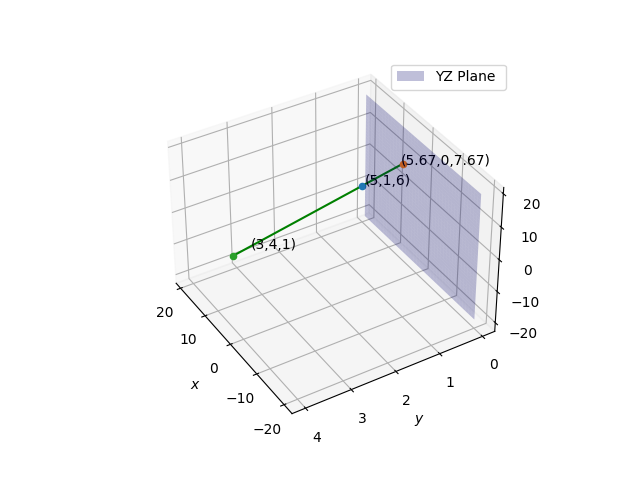
\includegraphics[ width=\columnwidth]{solutions/aug/2/37/figures/Line_AB.png}
\caption{Line and point of intersection}
\label{fig:Line }	
\end{figure}
